\section{Implementation \& Testing}

1. What to implement? Why implementing this function.

2. Description of the function to implement.

3. Test driven development, how to test? 

4. How to implement and improve performance?

- trick one

- trick two

... (see presentation)

5. Assembly optimisation

\begin{table}[h]
\centering

\begin{adjustbox}{max width=\textwidth}
\begin{tabular}{lccccccccccc}
\hline
	Function  & Total &&  \multicolumn{2}{c@{\hskip 0.2in}}{Polynomial arithmetics} && \multicolumn{2}{c}{Hash functions} && \multicolumn{2}{c}{Rest}\\\cline{4-5}\cline{7-8}\cline{10-11}
 
  & &&$k$ cycles & Percentage && $k$ cycles & Percentage && $k$ cycles & Percentage \\
 \hline
Key genration  & 5424 && 5082 & 93.6\% && 247 & 4.5\% && 95 & 1.7\% \\
Encryption & 1008 && 780 & 77.4\% && 160 & 15.9\% && 68 & 6.7\% \\
Decryption & 1757 && 1560 & 88.8\% & & 104 &5.9\% && 93 & 5.3\%  \\
\hline
\end{tabular}

\end{adjustbox}
\end{table}

%TODO add caption A Cost Breakdown (ref of the paper in mail) of Reference Code of NTRUEncrypt [4] (ref to ntru projet)

In fact as shown on table (add ref) the hash function takes up to 15.9\% of the total computation cycle number. It is the second most expensive operation after the polynomial arithmetics (that takes up to 93.6\% of the total cycle number). As shown on the table, the rest is negligible as it takes only up to 6.7\%. Hence the hash function $MGF-1$ is a good candidate for performance analysis in order to improve the global computation time by reducing the cycle number. Then, the project to realise was the implementation and optimisation of the $MGF-1$ function in $C$ according to the description of John Schanck \cite{schanck_practical_2015}. We implemented this function following a Test-driven development methodology. Thanks to the already existing implementation of NTRUOpenSourceProject\cite{noauthor_open_2018}, it was possible to compute the output of a predefined output and therefore to create test cases.

\begin{figure}[h]
  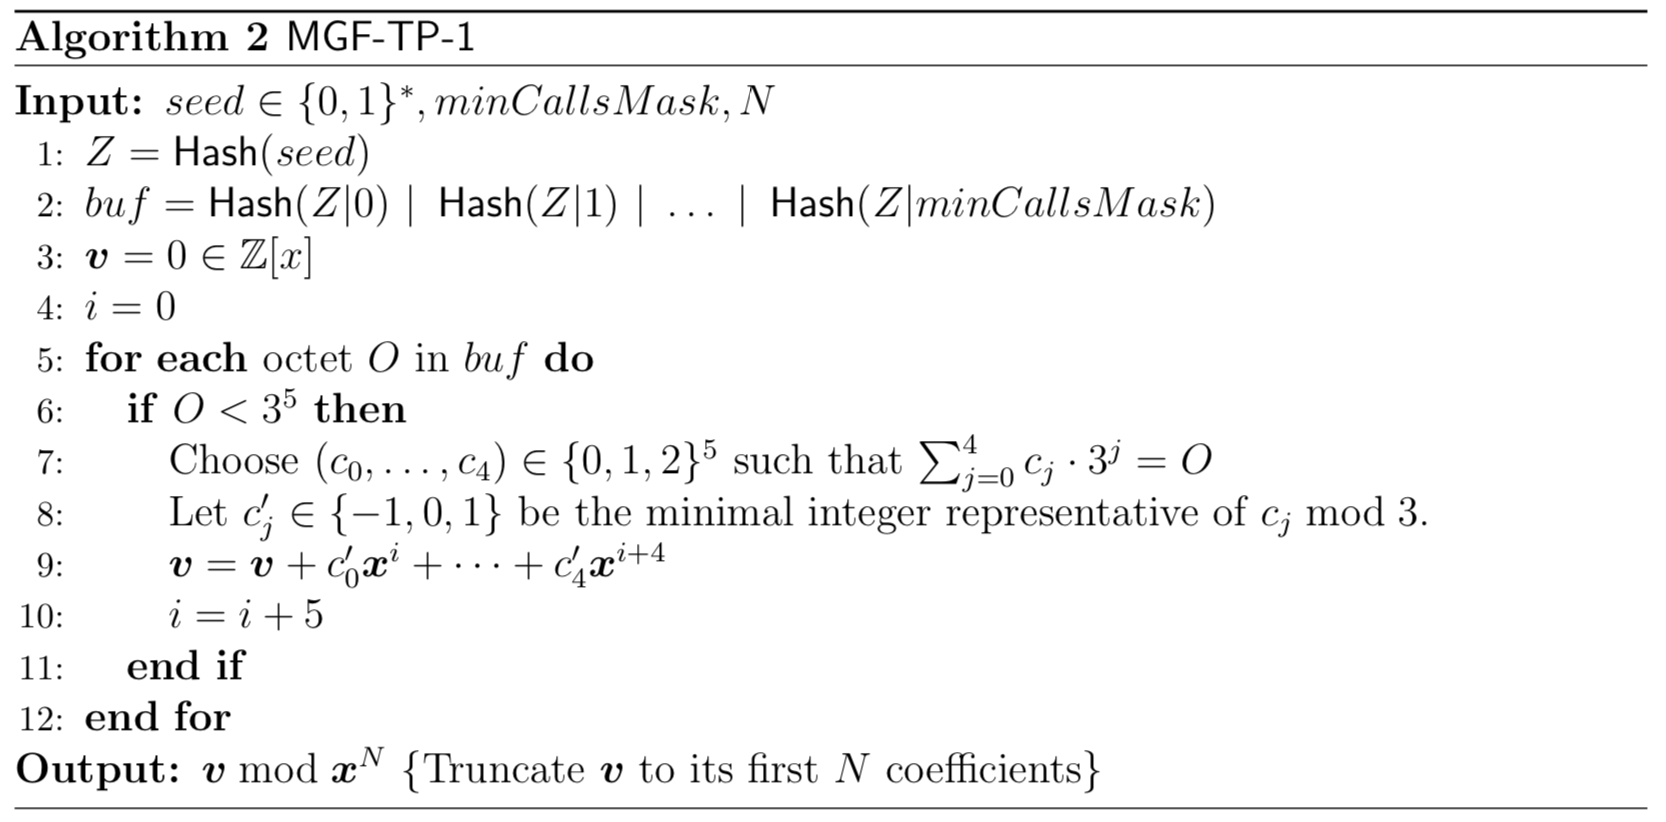
\includegraphics[width=\textwidth]{img/mgf1-description.png}
\end{figure}
% TODO: Add caption and ref to algo

